\documentclass{article}
\usepackage[utf8]{inputenc}
\usepackage{parskip} % Removes indent
\usepackage{amssymb} % Includes therefore symbol
\usepackage{amsmath} % Fractions 
\usepackage{array} % Formatting for tabular
\usepackage{graphicx} % Allows image inserting for the graph
\graphicspath{ {images/} } % Specifies folder location
\usepackage{subcaption} % For subfigure environment
\usepackage[export]{adjustbox} % Better image formatting
\usepackage{caption} % Needed to remove Figure prefix

\title{MAP4C Analyzing Two-Variable Data}
\author{Eric Taylor}
\date{May 2017}

\begin{document}

\topmargin=0pt % Sets top margin to 0pt
\headheight=0pt % Sets header distance to 0pt
\headsep=0pt % Sets distance between header and body to 0pt
\footskip=0pt % Sets footer to 0pt
\textheight=700pt % Sets height of body to 700pt

\setlength{\parindent}{0pt} % Removes indent

\captionsetup[figure]{labelformat=empty} % Removes Figure prefix from figure captions

\maketitle \thispagestyle{empty}

\textbf{{\huge Part 1}}

\textbf{\emph{\textsc{The Municipal Applied Practice College (or MAP College, for short) would like to construct a mathematical model that uses the grade 12 marks of incoming students to predict these same students' marks in their first-year of college. A comparison of these marks for a random sample of first year students is shown in the following table.}}}

\begin{tabular}{|l|l|l|l|l|l|l|l|l|l|l|}
    \hline \textbf{Grade 12 Average (\%)} & 78 & 85 & 75 & 76 & 81 & 79 & 82 & 74 & 80 & 83
    \\ \hline
    \textbf{First-Year Average (\%)} & 74 & 83 & 68 & 70 & 75 & 72 & 73 & 74 & 76 & 78 
    \\ \hline
\end{tabular} \\

\begin{center}
    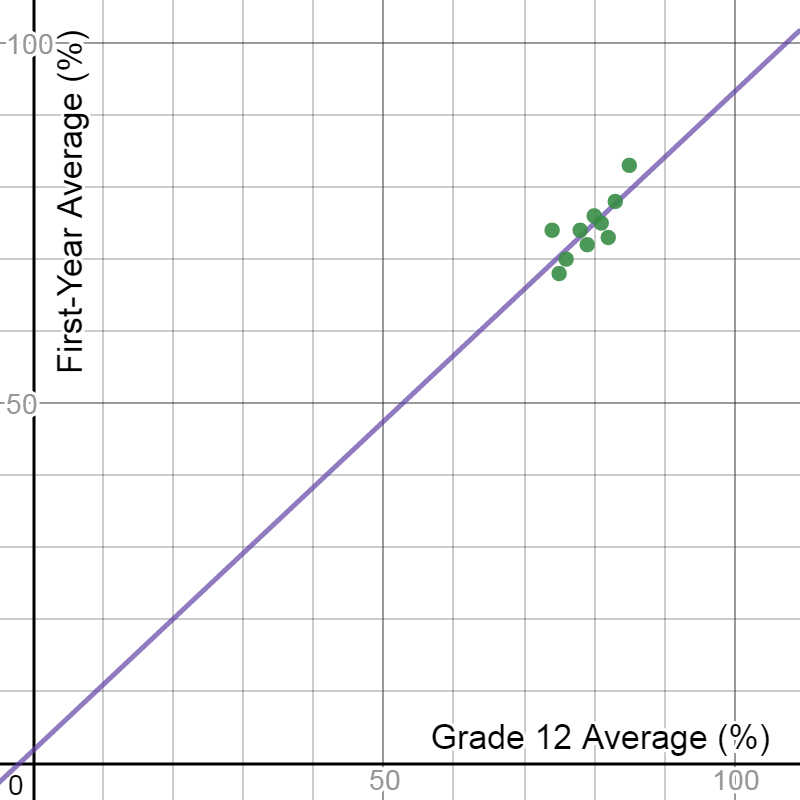
\includegraphics[width=8cm, height=5cm]{partone-graph}
\end{center}

\textbf{\emph{\textsc{1. Use Fathom to create a scatter plot for these data. Which variable should be placed on the x-axis? Why?}}}

The Grade 12 Average (\%) should be placed on the x-axis because it is the independent variable. The graph is using the Grade 12 Average (\%) to predict the college students' First-Year Average (\%), so it should be the base.

\newpage

\textbf{\emph{\textsc{2. Describe the correlation for this data, based on the scatter plot. Is there no correlation, positive correlation or negative correlation? If there is a correlation, is it strong or weak?}}}

There is a positive correlation as the values are positive and not declining. The correlation for this data is strong as the data points are closely clumped. 

\textbf{\emph{\textsc{3. Add a line-of-best-fit to the scatter plot and write the equation.}}}

(Refer to graph) \\
$y_{1}\mathtt{\sim}mx_{1}+b$ \\
$y_{1}\mathtt{\sim}0.913867*x_{1}+1.83032$

\textbf{\emph{\textsc{4. How well does the line-of-best-fit fit the data in the scatter plot? Justify your answer.}}}

The line-of-best-fit fits the data fairly well. There are an equal number of data points on each side of the line-of-best-fit, therefore there is equal distribution of data points.

\textbf{\emph{\textsc{5. Identify outliers, if any, and suggest possible reasons for an outlier.}}}

The range of all values is 68\% to 85\%. The grade 12 average is 79.3\% and the first year average is 67.3\%. You could argue that any percentage that is greater than or less than the average (by a reasonable percentage), or is outside the range, is an outlier. For sake of convenience, I will list outliers as any data point that is "far" from the line-of-best-fit. In this case, 85 is an outlier. Possible reasons for an outlier could be if the person did very well or very poorly in their grade 12 year or first college year, thus creating a gap.

\textbf{\emph{\textsc{6. Use the equation of the line-of-best-fit to predict the first-year average of a student with a grade 12 average of 81\%.}}}

The first-year average of a student with a grade 12 average of 81\% would be approximately 75.9\%. \\
$y_{1}\mathtt{\sim}mx_{1}+b$ \\
$y_{1}\mathtt{\sim}0.914*81+1.830$ \\
$y_{1}\mathtt{\sim}75.9$ \\

\newpage

\textbf{{\huge Part 2}}

\textbf{\emph{\textsc{Suzy is a student in the second year of her program at MAP College. She is starting to think about a job after graduation, and she is wondering about the job market as well as the starting salary she can expect to earn. Suzy does some research and finds employment statistics for graduates of her program and industry surveys of entry-level salaries. 300 students are expected to graduate from Suzy's program in 2011.}}}

\begin{tabular}{|m{8.5em}|m{8.5em}|m{8.5em}|m{8.5em}|}
    \hline \textbf{Year} & \textbf{Total Number of Graduates} & \textbf{Number Hired Upon Graduation} & \textbf{Mean Starting Salary (\$1000)}
    \\ \hline
    1997 & 218 & 185 & 28
    \\ \hline
    1998 & 205 & 180 & 30.5
    \\ \hline
    1999 & 192 & 168 & 30
    \\ \hline
    2000 & 220 & 188 & 32
    \\ \hline
    2001 & 218 & 208 & 33
    \\ \hline
    2002 & 225 & 184 & 32.5
    \\ \hline
    2003 & 232 & 185 & 34
    \\ \hline
    2004 & 238 & 193 & 37
    \\ \hline
    2005 & 249 & 198 & 38.5
    \\ \hline
    2006 & 266 & 209 & 40
    \\ \hline
\end{tabular}

\begin{figure}[h]
    \begin{subfigure}{0.5\textwidth}
        \begin{flushleft}
            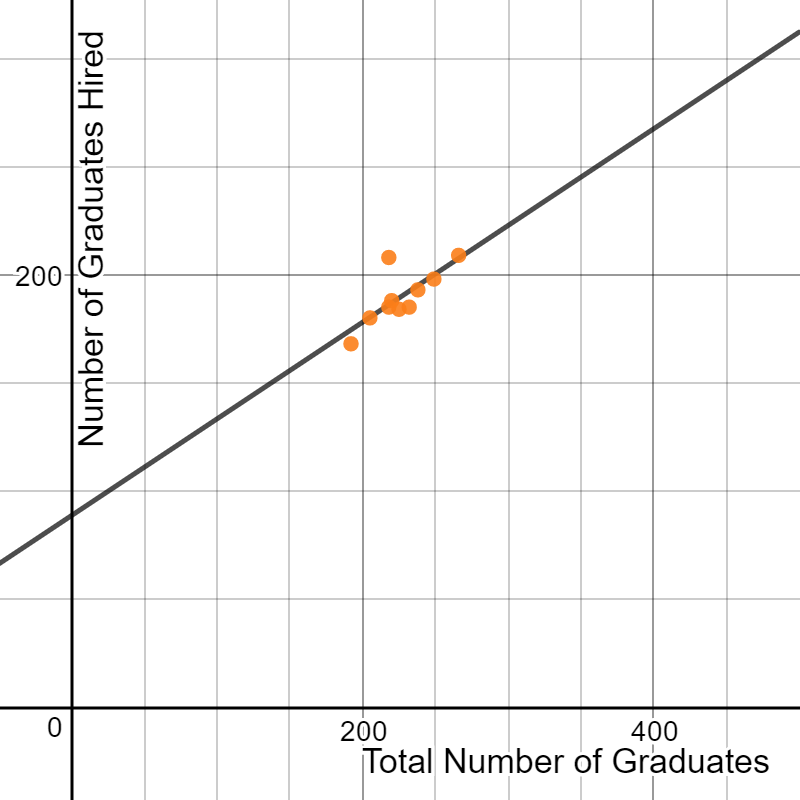
\includegraphics[width=6cm, height=5cm]{parttwo-graph-with-outlier}
            \caption{With outlier}
        \end{flushleft}
    \end{subfigure}
    \begin{subfigure}{0.5\textwidth}
        \begin{flushright}
            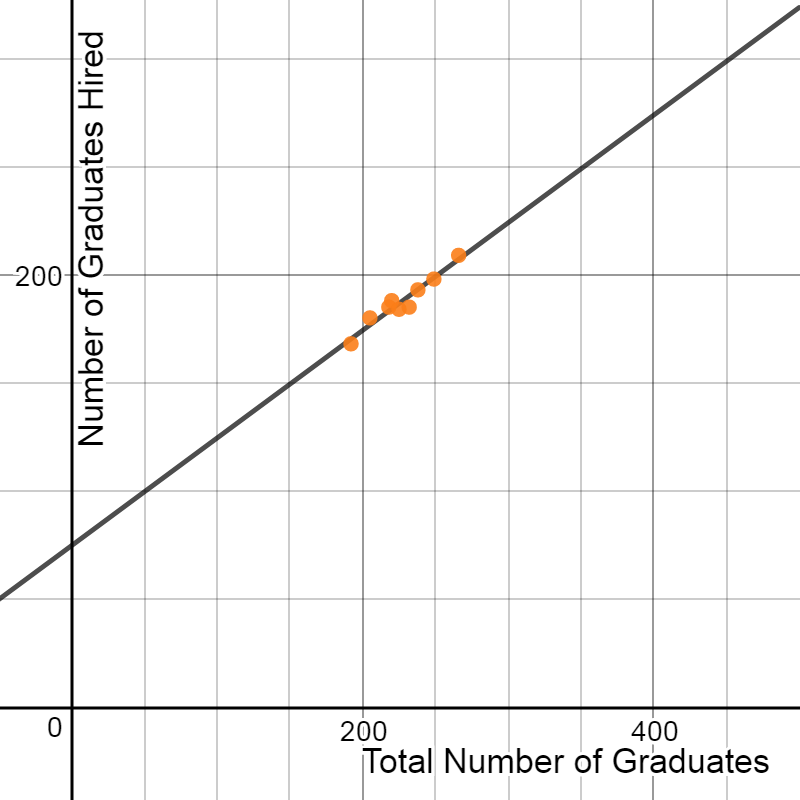
\includegraphics[width=6cm, height=5cm]{parttwo-graph-without-outlier}
            \caption{Without outlier}
        \end{flushright}
    \end{subfigure}
\end{figure}

\textbf{\emph{\textsc{1. Model the relationship between the total number of graduates and the number hired by creating a scatter plot and line-of-best-fit. Write the equation.}}}

(Refer to graph) \\
$y_{1}\mathtt{\sim}mx_{1}+b$ \\
$y_{1}\mathtt{\sim}0.447802*x_{1}+88.4623$

\newpage

\textbf{\emph{\textsc{2. How well does the line-of-best-fit fit the data in the scatter plot? Justify your answer.}}}

The line-of-best-fit fits the data fairly well. The line could be angled down slightly in order to divide the data points more equally. The outlier (218,208) is causing the line-of-best-fit to become the line-of-okay-fit because it is bringing it farther from the cluster.

\textbf{\emph{\textsc{3. Use the equation of this line-of-best-fit to predict how many graduates will be hired in 2011 if there are 300 graduates.}}}

The number of graduates that will be hired in 2011 if there are 300 graduates is approximately 223 graduates. \\
$y_{1}\mathtt{\sim}mx_{1}+b$ \\
$y_{1}\mathtt{\sim}0.447802*300+88.4623$ \\
$y_{1}\mathtt{\sim}223$

\textbf{\emph{\textsc{4. Identify any outliers in this scatter plot. List some reasons why the data could include an outlier. Do any of these reasons justify deleting the outlier from the scatter plot?}}}

An outlier in the scatter plot is (218,208). The data could include an outlier if there were an unusually high or low amount of graduates or graduates hired in a given year. Removing outliers is justified because they skew the data. They cause the line-of-best-fit to inaccurately represent the majority of data by pulling it farther away from the average.

\textbf{\emph{\textsc{5. Remove the outlier from the data. Create a new line-of-best-fit. Write the equation of this new line-of-best-fit.}}}

(Refer to graph) \\
$y_{1}\mathtt{\sim}mx_{1}+b$ \\ 
$y_{1}\mathtt{\sim}0.498414*x_{1}+74.527$

\textbf{\emph{\textsc{6. Use this new equation to recalculate the number of graduates that will be hired in 2011 if there are 300 graduates.}}}

The number of graduates that will be hired in 2011 if there are 300 graduates is approximately 224 graduates.

$y_{1}\mathtt{\sim}mx_{1}+b$ \\ 
$y_{1}\mathtt{\sim}0.498414*300+74.527$ \\
$y_{1}\mathtt{\sim}224$

\textbf{\emph{\textsc{7. Compare the results using the original line-of-best-fit and the new line-of-best-fit. Which result seems more reliable? Why?}}}

The new line-of-best-fit results seem more reliable because the exceptional case is removed. The data that is present is the best "average" sample, and provides a more accurate answer for the majority of cases.

\textbf{\emph{\textsc{8. Which of the two lines gives a more optimistic prediction for the number hired in 2011?}}}

The new line gives a more optimistic prediction for the number hired in 2011.

\textbf{\emph{\textsc{9. Are your calculations of graduates hired in 2011 an interpolation or an extrapolation? How do you know?}}}

My calculations of graduates hired in 2011 is an extrapolation because the 
data we are presuming is outside the data cluster. It is an estimation based on an extension of values we already have.

\newpage

\textbf{{\huge Part 3}}

\textbf{\emph{\textsc{1. List all possible combinations of two variables in the table that have not already been graphed}}}

\begin{tabular}{l l}
    Year \& Total number hired upon graduation & Year \& Total number of graduates 
    \\ 
    Total number of graduates \& Mean starting salary & Year \& Mean starting salary
    \\
    Number hired upon graduation \& Mean starting salary
\end{tabular}

\textbf{\emph{\textsc{2. Use Fathom to create scatter plots for 3 of the combinations listed above. Then, create a line-of-best-fit for each of the scatter plots. Print out all of your graphs.}}}

\begin{figure}[h]
    \begin{subfigure}{0.5\textwidth}
        \begin{flushleft}
            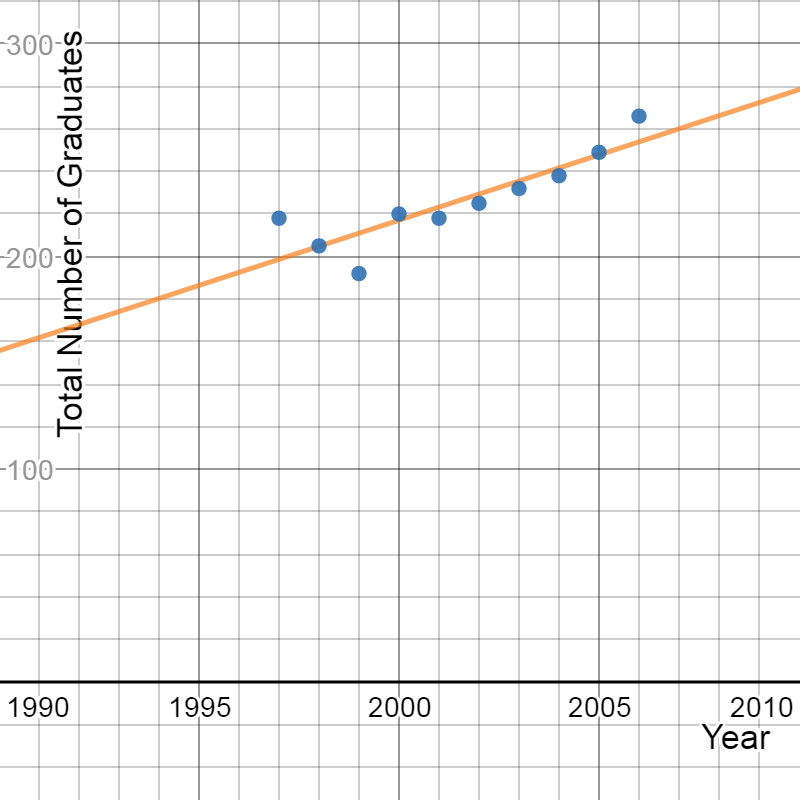
\includegraphics[width=5cm, height=5cm]{partthree-graph-yearandtotalgrad}
            \caption{Year \& Total number of graduates}
        \end{flushleft}
    \end{subfigure}
    \begin{subfigure}{0.5\textwidth}
        \begin{flushright}
            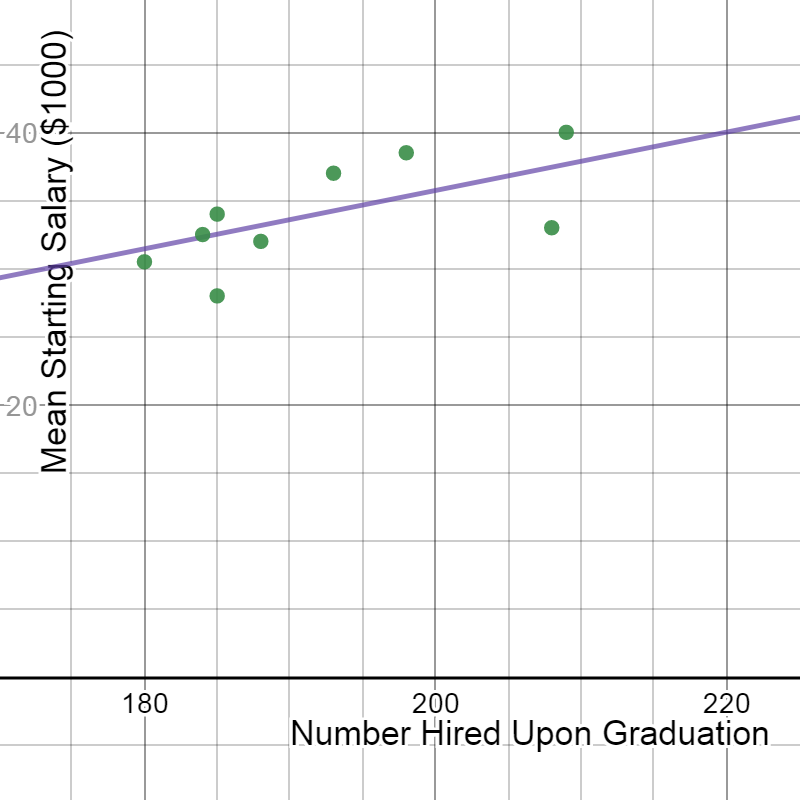
\includegraphics[width=6cm, height=5cm]{partthree-graph-numhiredandmeansalary}
            \caption{Number hired upon graduation \& Mean starting salary}
        \end{flushright}
    \end{subfigure}
\end{figure}
\begin{figure}[h]
        \begin{center}
            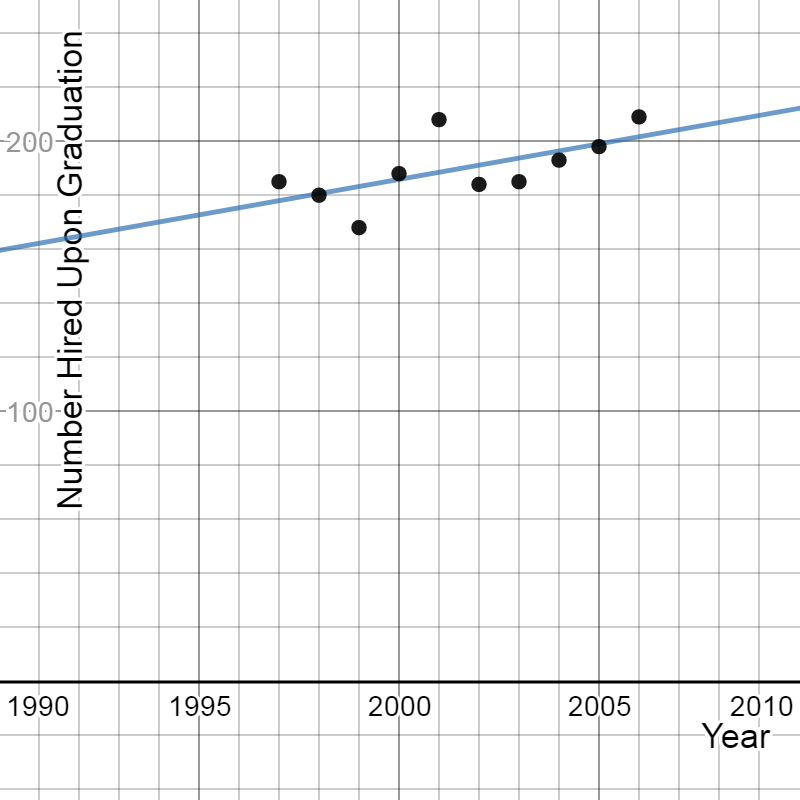
\includegraphics[width=6cm, height=5cm]{partthree-graph-yearandnumhired}
            \caption{(c) Year \& Number hired upon graduation}
        \end{center}
\end{figure}

\textbf{\emph{\textsc{3. Describe the correlation for each of the scatter plots. For example how strong is the relationship between the two variables chosen> For each graph, how well does the line-of-best-fit fit the data?}}}

Statistical correlation is measured by the coefficient of correlation, $r$; a positive $r$ value means that the correlation is positive, and a negative $r$ value means that the correlation is negative. An $r$ value greater than 0.5 and less than 1.0 means that the correlation is strong. Each graph has a positive $r$ value that is greater than 0.5, meaning that each graph has a strong, positive correlation. The line-of-best-fit fits the data in each graph very well, with the exception of graph b). Graph b) has many outliers, which pulls the line-of-best-fit away from the "true" best fit.




\end{document}
